\documentclass[12pt]{article}
\usepackage[utf8]{inputenc}
\usepackage[a4paper,margin=1in]{geometry}
\usepackage{amsmath,amssymb}
\usepackage{enumitem}
\usepackage{parskip}
\usepackage{xcolor}
\usepackage{fancyhdr}
\usepackage{tikz}
\usepackage{graphicx}
\usepackage{eso-pic}
\usepackage{titlesec}

\graphicspath{{../}}

\definecolor{kcpc-bg}{RGB}{250,250,250}
\definecolor{kcpc-text}{RGB}{20,20,20}
\definecolor{kcpc-muted}{RGB}{90,90,90}
\definecolor{kcpc-red}{RGB}{176,0,0}

\newcommand{\kcpcwordmark}{\raisebox{-0.15\height}{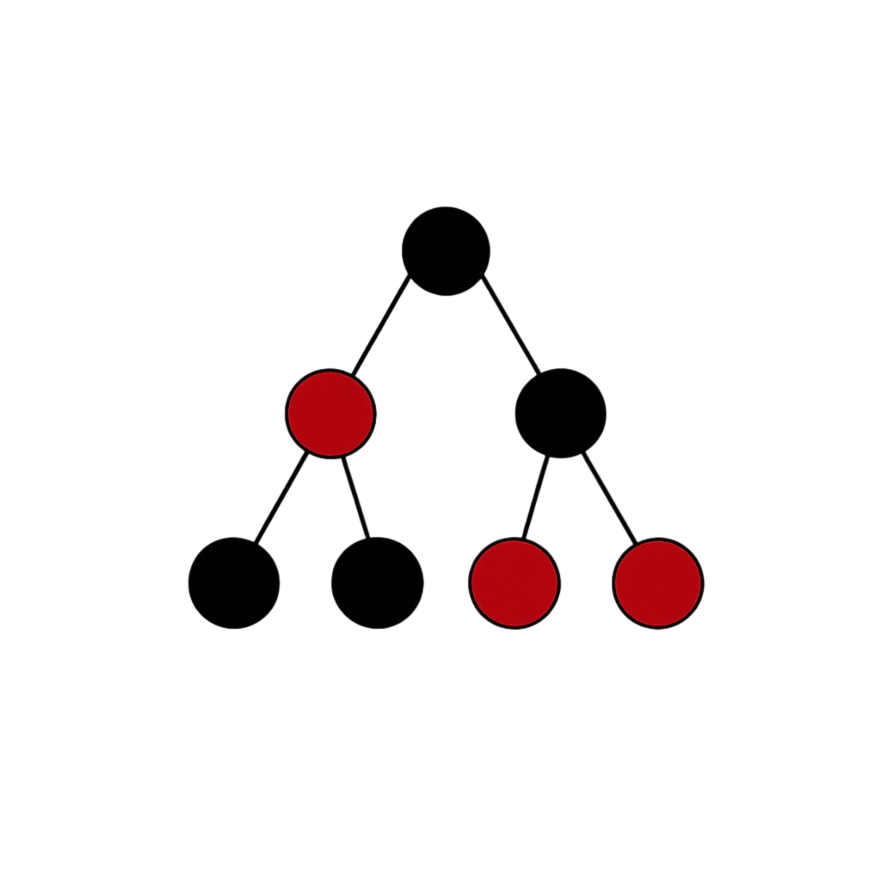
\includegraphics[height=0.55cm]{kcpc-logo.png}}}

\pagestyle{fancy}
\fancyhf{}
\lhead{\textcolor{kcpc-text}{\small\bfseries Solutions}}
\rhead{\textcolor{kcpc-muted}{\small Week 2}}
\cfoot{\textcolor{kcpc-muted}{\small KCPC}}
\renewcommand{\headrulewidth}{0.4pt}
\renewcommand{\headrule}{\hbox
to\headwidth{\color{kcpc-red}\leaders\hrule height \headrulewidth\hfill}}
\renewcommand{\footrulewidth}{0pt}
\setlength{\headheight}{28pt}

\AddToShipoutPictureBG{%
    \begin{tikzpicture}[remember picture,overlay]
        \node[opacity=0.035, at=(current page.center)]
        {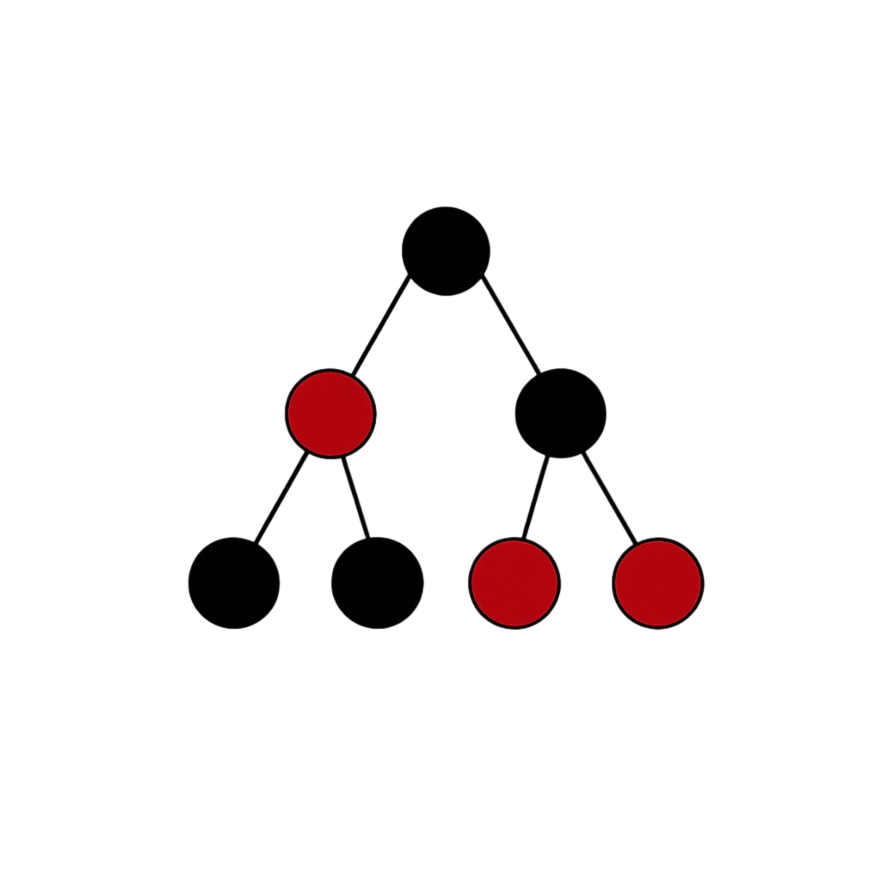
\includegraphics[width=0.38\paperwidth]{kcpc-logo.png}};
    \end{tikzpicture}%
}

\titleformat{\section}{\large\bfseries\color{kcpc-red}}{\thesection}{1em}{}

\setlist[itemize]{noitemsep, topsep=4pt}
\setlist[enumerate]{topsep=4pt}

\newcommand{\insight}[1]{\par\medskip\noindent\textbf{Key insight:} #1}

\title{KCPC Week 2 Solutions}
\author{}
\date{}

\begin{document}
\maketitle
\thispagestyle{fancy}

\section{Wishful Thinking}

\subsection*{Basic -- Complete The Square}
Subtract the right-hand side from the left:
\[
x^2+y^2-\frac{(x+y)^2}{2}=\frac{(x-y)^2}{2}\ge0.
\]
Equality holds exactly when $x=y$.
\insight{Wish for a square because squares are automatically non-negative.}

\subsection*{Easy -- Make The Sum Telescope}
Use partial fractions:
\[
\frac1{k(k+1)}=\frac1k-\frac1{k+1}.
\]
Therefore all intermediate terms cancel:
\[
\sum_{k=1}^{n}\left(\frac1k-\frac1{k+1}\right)
=1-\frac1{n+1}=\frac n{n+1}.
\]
\insight{Rewriting each term as a difference exposes cancellation.}

\subsection*{Medium -- A Number Puzzle}
Set $x=u+v$ and $y=u-v$. The equation becomes
$u^2+v^2=z^2$. Take the Pythagorean triple
\[
u=m^2-1,\qquad v=2m,\qquad z=m^2+1
\]
for any integer $m\ge3$. Then
\[
x=m^2+2m-1,\qquad y=m^2-2m-1,\qquad z=m^2+1
\]
is positive and satisfies the original equation. Varying $m$ gives
infinitely many solutions.
\insight{The substitution turns the desired equation into a familiar one.}

\subsection*{Hard -- Improve The Recurrence}
Define $b_n=a_n+1$. Then
\[
b_{n+1}=a_{n+1}+1=2a_n+2=2b_n,
\qquad b_1=2.
\]
Hence $b_n=2^n$, so
\[
a_n=2^n-1.
\]
\insight{Changing variables absorbs the awkward constant term.}

\subsection*{Very Hard -- Factor The Equation}
Multiplying by $nxy$ gives $n(x+y)=xy$. Rearranging and adding $n^2$
to both sides gives
\[
(x-n)(y-n)=n^2.
\]
Both $x$ and $y$ must exceed $n$. Thus, for every positive divisor
$d$ of $n^2$, set
\[
x=n+d,\qquad y=n+\frac{n^2}{d}.
\]
These are all ordered positive solutions, since every factorisation
of $n^2$ arises this way.
\insight{Adding the right term changes a sum equation into a factorisation.}

\section{Symmetry}

\subsection*{Basic -- Chomp: Poisoned Chocolate}
Suppose the second player has a winning strategy. If the first player
eats only the top-right square, this strategy specifies a reply at
some unpoisoned square $q$. The first player could instead have chosen
$q$ as their opening move: every move at $q$ also eats the top-right
square, so the resulting board is exactly the board after those two
hypothetical moves. It is now the second player's turn, whereas in the
hypothetical game it was the first player's turn. The first player
can therefore take over the supposed winning \emph{second-player}
strategy, a contradiction. Thus the first player has a winning
strategy, although this argument does not specify their first move.
\insight{A hypothetical winning reply can be stolen as the first move.}

\subsection*{Easy -- Coins On A Circular Table}
The first player places a coin at the centre. After every later move,
the first player places a coin in the position obtained by rotating
the opponent's coin by $180^\circ$. The table remains symmetric after
each response, so the mirrored placement is legal whenever the
opponent's placement is legal. The first player therefore moves last.
\insight{Occupy the unique fixed point, then pair all remaining positions.}

\subsection*{Medium -- A Symmetric Integral}
Let $I=\int_0^1f(x)\,dx$. Substituting $u=1-x$ gives
\[
I=\int_0^1f(1-x)\,dx.
\]
Adding the two expressions and using the given identity,
\[
2I=\int_0^1\bigl(f(x)+f(1-x)\bigr)\,dx=\int_0^1 1\,dx=1.
\]
Hence $I=\tfrac12$.
\insight{Reflecting the interval pairs every value with its complement.}

\subsection*{Hard -- Odd Skew-Symmetric Matrices}
Using invariance of the determinant under transposition,
\[
\det A=\det A^{\mathsf T}=\det(-A)=(-1)^n\det A.
\]
When $n$ is odd this says $\det A=-\det A$, so $2\det A=0$ and
$\det A=0$.
\insight{Transpose symmetry turns the determinant into its own negative.}

\subsection*{Very Hard -- Six People}
Represent people by vertices and colour each edge red for acquaintances
and blue for strangers. Choose a vertex $v$. At least three of its
five incident edges have one colour; by symmetry suppose $va,vb,vc$
are red. If one of $ab,bc,ca$ is red, it forms a red triangle with
$v$. Otherwise $ab,bc,ca$ are all blue and form a blue triangle.
\insight{Colour symmetry reduces two relationship cases to one.}

\section{Extreme Principle}

\subsection*{Basic -- Erd\H{o}s--Szekeres Monotone Subsequence}
For each term $a_i$, let $L_i$ be the length of the longest increasing
subsequence starting at $a_i$, and $D_i$ the longest decreasing. If
$a_i<a_j$ with $i<j$, then $L_i>L_j$; if $a_i>a_j$, then $D_i>D_j$.
Thus all pairs $(L_i,D_i)$ are distinct. Each $L_i,D_i$ is between 1
and $n$ (otherwise we have the desired subsequence). There are at most
$n^2$ distinct pairs, but $n^2+1$ terms. By pigeonhole, some pair
repeats, contradiction unless a subsequence of length $n+1$ exists.
\insight{Map each term to a pair of lengths; pigeonhole principle forces a collision unless the bound is reached.}

\subsection*{Easy -- Minimum Degree Forces A Cycle}
Choose a longest path $v_0v_1\ldots v_k$. Every neighbour of $v_k$
must already lie on the path, since a new neighbour would extend it.
Because $v_k$ has at least two neighbours, it is adjacent to some
$v_i$ with $i<k-1$. The edge $v_kv_i$ together with the path from
$v_i$ to $v_k$ forms a cycle.
\insight{An endpoint of a longest path cannot escape to a new vertex.}

\subsection*{Medium -- An Empty Triangle}
Among all non-degenerate triangles whose vertices belong to the set,
choose one of minimum positive area. If another given point lay in
its interior, joining that point to the three vertices would split
the triangle into three smaller triangles of positive area. At least
one would contradict the chosen minimum. Therefore its interior is empty.
\insight{A minimum-area counterexample cannot contain a smaller one.}

\subsection*{Hard -- A Path Through A Tournament}
Choose a longest directed path $v_1\to\cdots\to v_k$. Suppose a
vertex $u$ is omitted. If $u\to v_1$, prepend $u$; if $v_k\to u$,
append $u$. Otherwise $v_1\to u$ and $u\to v_k$. Moving along the
path, there is an index $i$ with $v_i\to u$ and $u\to v_{i+1}$, so
$u$ can be inserted between them. Every case contradicts maximality,
so the path contains every vertex.
\insight{A longest object is rigid enough that an omitted vertex causes a contradiction.}

\subsection*{Very Hard -- Longest Paths Meet}
Let two longest paths $P$ and $Q$ both have $L$ edges. Suppose they
are disjoint. Since the graph is connected, choose a shortest path
joining a vertex $p$ of $P$ to a vertex $q$ of $Q$, with no other
vertices on $P\cup Q$. From $p$, one endpoint of $P$ is at distance
at least $L/2$ along $P$; similarly, one endpoint of $Q$ is at
distance at least $L/2$ from $q$. Joining these two subpaths through
the connecting path produces a path longer than $L$, a contradiction.
\insight{Two disjoint extremes can be joined to create something more extreme.}

\section{Reduction}

\subsection*{Basic -- An Acquaintance Graph}
Represent each person by a vertex and join two vertices when those
people are acquainted. Every degree is one of $0,1,\ldots,n-1$.
However, degrees 0 and $n-1$ cannot both occur: if one person knows
everyone, nobody knows zero people. Thus at most $n-1$ different
degree values occur among $n$ vertices. By the pigeonhole principle,
two vertices have the same degree.
\insight{The graph representation turns acquaintances into vertex degrees.}

\subsection*{Easy -- The Bridges Of K\"onigsberg}
Replace each land mass by a vertex and each bridge by an edge. A walk
using every bridge exactly once would be an Euler trail. In such a
trail, every vertex except possibly the start and finish has even
degree. The K\"onigsberg graph has four odd-degree vertices, so no
Euler trail exists.
\insight{Only incidence matters, so geography can be discarded.}

\subsection*{Medium -- Missionaries And Cannibals}
State: $(M_L,C_L,B)$ with $M$ missionaries, $C$ cannibals on left,
$B\in\{L,R\}$ boat position. On each bank, safety requires that
there are no missionaries or that missionaries are at least as
numerous as cannibals. Graph edges are valid crossings with one or
two passengers. A BFS from $(3,3,L)$ to $(0,0,R)$ gives the following
11 crossings (\texttt{M} = missionary, \texttt{C} = cannibal):
\[
\begin{gathered}
\texttt{CC}\to,\quad \texttt{C}\leftarrow,\quad
\texttt{CC}\to,\quad \texttt{C}\leftarrow,\quad
\texttt{MM}\to,\quad \texttt{MC}\leftarrow,\\
\texttt{MM}\to,\quad \texttt{C}\leftarrow,\quad
\texttt{CC}\to,\quad \texttt{C}\leftarrow,\quad
\texttt{CC}\to.
\end{gathered}
\]
Checking the counts on each bank after every crossing shows that
none ever leaves a missionary outnumbered.
\insight{State-space graph with safety constraints; BFS finds valid path.}

\subsection*{Hard -- Lamps As Linear Algebra}
Encode on/off by $1/0$ in $\mathbb F_2$. Let $v$ be the initial state
and let column $i$ of an $n\times n$ matrix $A$ have ones in positions
$i-1,i,i+1$ modulo $n$. If $x_i$ records whether move $i$ is used,
then reaching all off is equivalent to
\[
Ax=v\quad\text{over }\mathbb F_2.
\]
Gaussian elimination decides whether this system is consistent and,
when it is, returns a sequence of moves. Repeating a move is unnecessary
because doing it twice has no effect.
\insight{Toggle operations become vector addition modulo 2.}

\subsection*{Very Hard -- Assignment As Maximum Flow}
Create a source $s$, one vertex for each student, one for each project,
and a sink $t$. Add capacity-1 edges from $s$ to every student, from
a student to each acceptable project, and from every project to $t$.
An integral flow of value $n$ selects one outgoing student--project
edge for every student and uses every project at most once. Conversely,
any valid assignment gives such a flow. Therefore an assignment exists
exactly when the maximum flow has value $n$.
\insight{Capacity constraints encode distinct choices, reducing assignment to flow.}

\newpage
\section*{Advanced Material}
The remaining solutions cover optional extensions. Their theory and
worked examples are presented in \textit{Week 2 Advanced Slides}.

\section{Advanced Logic And Common Knowledge}

\subsection*{Basic -- Blue-Eyed Islanders ($k=2$)}
If $k=1$, the single blue-eyed islander sees no blue eyes, knows the
announcement refers to them, and leaves night 1.
If $k=2$, each blue-eyed islander sees one blue-eyed person. If I had
brown eyes, the other would see 0 blue eyes and leave night 1. They
don't. So I must have blue eyes. Both leave night 2.
\insight{Public announcement creates common knowledge; induction on
$k$ gives the day of departure.}

\subsection*{Easy -- Cheating Husbands}
Let $k$ be the number of cheating husbands. By the same induction as
Blue-Eyed Islanders, all $k$ wives deduce their husbands cheated on
day $k$ and act at midnight. The queen's truthful announcement
ensures that $k\ge1$.

\subsection*{Medium -- Sum And Product Puzzle}
The information limit $x+y\le100$ makes systematic elimination
possible. Start with all pairs
$\Omega_0=\{(x,y):2\le x<y,\ x+y\le100\}$. Keep in $\Omega_1$
only pairs whose product occurs for \emph{at least two} pairs in
$\Omega_0$ (P's first statement). Keep in $\Omega_2$ only pairs for
which \emph{every} $\Omega_0$ pair with the same sum belongs to
$\Omega_1$ (S knew P could not know). The possible sums in
$\Omega_2$ are
\[
11,17,23,27,29,35,37,41,47,53.
\]
Keep in $\Omega_3$ only pairs whose product occurs \emph{once} in
$\Omega_2$ (P now knows). Finally keep in $\Omega_4$ only pairs
whose sum occurs \emph{once} in $\Omega_3$ (S now knows). Enumerating
the pairs under the given bound yields $\Omega_4=\{(4,13)\}$.
For example, product 52 has factor pairs $(2,26)$ and $(4,13)$;
only the latter has a sum surviving S's first statement. The answer
is $x=4$, $y=13$. These filters spell out exactly which set of
possibilities each speaker has at every stage.
\insight{Filter a finite set of possible worlds after each public statement.}

\subsection*{Hard -- Cheryl's Birthday}
Dates: May 15, 16, 19; June 17, 18; July 14, 16; Aug 14, 15, 17.
Albert knows month, Bernard knows day.
Albert: Bernard doesn't know $\to$ month is not May or June (19 and
18 are unique days). Remaining: July 14, 16; Aug 14, 15, 17.
Bernard now knows $\to$ day is not 14. Remaining: July 16; Aug 15, 17.
Albert now knows $\to$ month must be July (if August, Albert couldn't
distinguish 15 and 17). Answer: July 16.

\subsection*{Very Hard -- 100 Prisoners And A Light Bulb}
Designate one prisoner as the Counter. Others are Drones.
Protocol: A Drone who has never turned the light on, and finds it
off, turns it on exactly once. The Counter only turns the light off,
and increments a mental count each time they find it on. When the
Counter's count reaches 99, they announce.
Proof: Each Drone eventually visits and turns the light on if they
haven't, with probability 1: independent uniform visits give each
prisoner infinitely many opportunities. Each on-state waits until
the Counter next visits, at which point they turn it off and record
the signal. Consequently all 99 Drones eventually signal, and the
count reaches 99 exactly when all 99 have visited. Every announcement
is correct, and the protocol terminates almost surely.
\insight{The light bulb encodes one bit of shared state; the Counter
aggregates information.}

\section{Advanced Invariants And Monovariants}

\subsection*{Basic -- Peg Solitaire (Small Board)}
No legal first move exists. The centre is the only empty cell, but
an orthogonal jump landing there would have to start two squares away
from the centre, outside the $3\times3$ board. Thus the initial
configuration is already stuck with eight pegs.
\insight{Check whether a first move exists before seeking a more elaborate invariant.}

\subsection*{Easy -- Token Game}
Initially the only adjacent pair is at 0 and 1, so the only move
replaces those two tokens with one token at 2. No further move is
possible with just one token. Position 100 is never occupied.

\subsection*{Medium -- Conway's Soldiers}
Fix a possible target square $(x_0,5)$ and put
$\varphi=(\sqrt5-1)/2$, so $\varphi+\varphi^2=1$.
Assign cell $(x,y)$ weight $\varphi^{|x-x_0|+|y-5|}$.
For any three consecutive cells in a row or column, the weight of
the destination is at most the sum of the weights of the two cells
from which a peg jumps. In the only tight case, their distances from
the target are $k+2,k+1,k$ and the inequality is precisely
$\varphi^{k+2}+\varphi^{k+1}=\varphi^k$.
Removing the jumped peg therefore never increases total weight.

The initially occupied cells have total weight exactly 1:
\[
\sum_{y\le0}\sum_{x\in\mathbb Z}
\varphi^{|x-x_0|+5-y}
=\frac{\varphi^5}{1-\varphi}
 \left(1+\frac{2\varphi}{1-\varphi}\right)=1.
\]
The target itself has weight 1. After any finite number of jumps,
infinitely many initial pegs remain elsewhere, with positive total
weight. Reaching the target would give total weight greater than 1,
a contradiction. This holds for every $x_0$, so row 5 is unreachable.

\subsection*{Hard -- Polynomial Invariant For (x+2,y-1)}
The move $(x,y)\to(x+2,y-1)$ changes $x+2y$ by $2+2(-1)=0$. Thus
$P(x,y)=x+2y$ is a polynomial invariant. More generally, any
polynomial in $x+2y$ is invariant. This is a \emph{necessary} condition
for reachability, not sufficient: the move can only be applied a
non-negative integer number $k$ of times. The exact reachable set
is $\{(2k,-k):k\in\mathbb Z_{\ge0}\}$, which lies on the line
$x+2y=0$.
\insight{An invariant excludes states, while the direction of the move
and integrality complete the reachability argument.}

\subsection*{Very Hard -- A Sequence Invariant}
Set $b_n=a_n+1$. The given recurrence becomes the Fibonacci-type
recurrence $b_{n+1}=b_n+b_{n-1}$, with $b_0=1$, $b_1=2$ and $b_2=3$.
For $d_n=b_n^2-b_{n-1}b_{n+1}$,
\[
\begin{aligned}
d_{n+1}&=b_{n+1}^2-b_nb_{n+2}\\
&=b_{n+1}(b_n+b_{n-1})-b_n(b_{n+1}+b_n)\\
&=b_{n+1}b_{n-1}-b_n^2=-d_n.
\end{aligned}
\]
Since $d_1=b_1^2-b_0b_2=4-3=1$, we have
$d_n=(-1)^{n-1}$, proving the claimed invariant.

\section{Colouring And Tiling: Generalisations}

\subsection*{Basic -- Mutilated Chessboard: Four Corners Removed}
Yes. In each of the top and bottom rows, the two corners are missing,
leaving six consecutive squares; tile each row with three horizontal
dominoes. Each of the other six rows has eight squares and can be
tiled with four horizontal dominoes. These $3+3+6\cdot4=30$ dominoes
cover every remaining square.
\insight{An explicit tiling is more decisive than an unnecessary colouring.}

\subsection*{Easy -- Tiling With T-Tetrominoes}
The equal letters in this diagram give four T-shaped pieces:
\begin{center}
\begin{verbatim}
AAAB
CABB
CCDB
CDDD
\end{verbatim}
\end{center}
Each letter appears in four edge-connected cells forming a T. To
tile $4\times(4k)$, divide it into $k$ disjoint $4\times4$ blocks and
repeat this construction in every block.

\subsection*{Medium -- Fault-Free Domino Tiling}
For a $6\times6$ board, consider any one of its five internal
horizontal grid lines. The number of vertical dominoes crossing it
must be even: the part above the line has an even number of cells,
and all other dominoes cover two cells there. If the tiling is
fault-free, at least two dominoes cross each such line. The same
argument applies to its five internal vertical lines. Since each
domino crosses at most one grid line, fault-freeness would require
at least $2(5+5)=20$ dominoes, but the board holds only 18.

Here is a fault-free $6\times8$ tiling; each repeated letter is one
domino, and the paired cells are adjacent:
\begin{center}
\begin{verbatim}
AABBCCDE
FFGGHIDE
JKKLHIMM
JNOLPPQQ
RNOSSTTU
RVVWWXXU
\end{verbatim}
\end{center}
Every one of the five internal horizontal and seven internal vertical
lines crosses a domino, so there is no fault line.

\subsection*{Hard -- Triominoes On A Chessboard}
Choose row and column indices starting at the removed corner, and
colour $(i,j)$ by $(i+j)\bmod3$. Every horizontal or vertical
$1\times3$ tromino covers one cell of each colour. The intact board
has colour counts $21,22,21$; removing the $(0,0)$ corner leaves
$20,22,21$, which are not equal. Therefore no tiling exists.

\subsection*{Very Hard -- Generalised Mutilated Chessboard}
The answer is $m,n\ge2$ with $mn$ even, together with the two boards
$1\times2$ and $2\times1$ (whose empty remainder has an empty tiling).
Odd area leaves an odd number of squares and cannot be tiled. For
$m,n\ge2$ with even area, rotate the board if necessary so that its
number of rows is even. Cross the top row from left to right, snake
through columns $2$ through $n$ of the remaining rows, then return
up column $1$. This is a Hamiltonian cycle of the board's squares.
Colours alternate around the cycle; deleting two opposite-colour
squares leaves two paths, each containing an even number of squares.
Pair consecutive squares on each path to tile the remainder.

Finally, on a $1\times n$ board of even length $n\ge4$, remove
positions 2 and 3. They have opposite colours but leave position 1
isolated, so this board does not \emph{always} admit a tiling. The
same holds after rotation. The $1\times2$ case is the sole exception.

\section{Induction And Recursion: From Proof To Algorithm}

\subsection*{Basic -- Josephus Problem}
$J(1)=1$. Number the people $1$ through $n$ and start by removing
person 2. For $2k$ people, the first circuit removes every even
position; the $k$ odd-numbered survivors form a smaller Josephus
circle, giving $J(2k)=2J(k)-1$. For $2k+1$ people, the first circuit
removes $2,4,\ldots,2k$ and then person 1. The remaining $k$ people
are $3,5,\ldots,2k+1$, giving $J(2k+1)=2J(k)+1$.
These recurrences imply by induction that if $n=2^r+s$ with
$0\le s<2^r$, then $J(n)=2s+1$: for even and odd $n$ alike, the
formula for $J(\lfloor n/2\rfloor)$ gives the next case.
Equivalently, move the leading bit of $n$'s binary representation
to the end.

\subsection*{Easy -- Gray Codes}
$G_1 = [0,1]$. Given $G_n$, construct $G_{n+1}$ by prefixing 0 to
$G_n$ and prefixing 1 to reverse of $G_n$. Proof by induction:
consecutive strings in first half differ by induction; boundary
between halves is $0w$ followed by $1w$, where $w$ is the last
string of $G_n$, so only the first bit changes. Consecutive strings
in the reversed second half also differ by induction, and every
$(n+1)$-bit string appears exactly once.

\subsection*{Medium -- Recursive 15-Puzzle Parity}
Read the numbered tiles row by row, omitting the blank, and count
inversions $I$. Let $r$ be the blank's row counted from the bottom,
starting at 1. A horizontal move leaves both parities unchanged; a
vertical move changes $r$ by 1 and changes inversion parity by 3.
Thus $I+r$ has invariant parity. The goal has $I=0,r=1$, so a
configuration is solvable \emph{only if} $I+r$ is odd. To obtain a
self-contained recursive decision algorithm without assuming the
converse, reject even-parity configurations, then recursively explore
legal slides from an odd-parity configuration using depth-first
search and a visited-state set. Return true on reaching the goal;
return false if all reachable states have been explored. There are
finitely many arrangements, and every legal path is explored, so this
algorithm terminates and answers correctly. Count inversions by
recursively splitting the list in two, counting inversions in each
half and cross-inversions while merging. The parity check takes
$O(16\log16)$ time; exhaustive search is much more expensive.

\subsection*{Hard -- Counterfeit Coin With $n$ Weighings}
The answer, for $n\ge2$ and no initially known genuine coin, is
$N_n=(3^n-3)/2$. The following two auxiliary strategies explain how
to attain it.

\emph{Signed suspects:} If each of $3^r$ suspect coins has a known
direction (it can only be heavy or only be light), $r$ weighings
suffice. For $r=0$ there is one suspect. For the induction step put
$t=3^{r-1}$, and, by reversing heavy/light if needed, let at least
half of the $3t$ suspects be heavy candidates. If at least $2t$
are heavy candidates, weigh $t$ heavy candidates against $t$ others:
balance leaves $t$ suspects, while a tilt selects the $t$ heavy
candidates on the heavier pan. Otherwise put $(t+1)/2$ heavy and
$(t-1)/2$ light candidates on \emph{each} pan. A balance leaves $t$
suspects off the scale; a tilt leaves the heavy candidates on the
heavier pan and the light candidates on the lighter pan, again $t$
in all. Each case reduces to the induction hypothesis.

\emph{Known genuine coin:} With a genuine reference, we can resolve
$U_r=(3^r-1)/2$ unknown suspects in $r$ weighings. For $r=1$,
compare the suspect with the genuine coin. For $r>1$, let
$t=3^{r-1}$; weigh $(t+1)/2$ suspects against $(t-1)/2$ other suspects
and one genuine coin. If balanced, $U_{r-1}$ unweighed suspects
remain, still with a genuine reference. If tilted, the $t$ weighed
suspects have known heavy/light directions and the signed-suspect
strategy applies.

Now split $N_n=3U_{n-1}$ unknown coins into equal groups $A,B,C$
and weigh $A$ against $B$. If balanced, $C$ contains the counterfeit
and $A$ supplies genuine coins, so use the known-genuine strategy.
If tilted, a coin in the heavier group might be heavy \emph{or} one
in the lighter group might be light. These are $2U_{n-1}=3^{n-1}-1$
signed suspects; add one known genuine coin from $C$ as a dummy
candidate and apply the signed-suspect strategy. The dummy cannot be
the answer. This constructs a strategy in $n$ weighings.

For optimality, suppose the first weighing compares $k$ unknown
coins against $k$ others, leaving $N-2k$ off the scale. A tilt gives
$2k$ signed possibilities and only $3^{n-1}$ remaining outcome
sequences; as $2k$ is even, $2k\le3^{n-1}-1$. A balance gives genuine
coins but $N-2k$ unknown ones, so the known-genuine bound gives
$N-2k\le U_{n-1}$ (the all-balanced outcome cannot distinguish the
two directions of an unweighed counterfeit). Hence
$N\le(3^{n-1}-1)+U_{n-1}=(3^n-3)/2$.

\subsection*{Very Hard -- Hadamard Matrix Construction}
$H_1=[1]$. $H_{2n}=
\begin{bmatrix}H_n & H_n\\H_n & -H_n
\end{bmatrix}$.
Proof: Rows of $H_{2n}$ are either $(r,r)$ or $(r,-r)$ for rows $r$
of $H_n$. Orthogonality follows from orthogonality of $H_n$ rows. By
induction, $H_{2^k}$ is Hadamard.

\section{Algorithmic Bridges}

\subsection*{Basic -- A Maze As A Graph}
Create one vertex for every open cell. Join two vertices when their
cells share a side. Run BFS from the start, storing distance 0 there
and assigning each newly discovered neighbour distance one greater
than its parent. The finish distance is the minimum number of moves;
if it is never discovered, no route exists. BFS is optimal because it
visits vertices in non-decreasing distance from the start, so the
first path reaching any cell uses the fewest possible edges.

\subsection*{Easy -- Greedy Activity Selection}
Sort by finish time $f_1\le f_2\le\cdots\le f_n$. Pick $i_1=1$. For
$k>1$, pick first $i_k$ with $s_{i_k}\ge f_{i_{k-1}}$.
Proof by exchange: let $O$ be an optimal solution with earliest first
finish. If $O$ doesn't pick the greedy first choice, exchange it; the
new solution is at least as good and has earlier first finish. Repeat
inductively.

\subsection*{Medium -- DP From Induction: Coin Change}
$f(s)=$ min coins to make sum $s$. Recurrence: $f(s)=1+\min_{c_i\le
s} f(s-c_i)$, with $f(0)=0$, $f(s<0)=\infty$.
Tabulation: for $s=1$ to $n$, for each coin $c_i\le s$, update
$f(s)=\min(f(s), 1+f(s-c_i))$. Time $O(kn)$, space $O(n)$.

\subsection*{Hard -- Sliding Puzzle State-Space Search}
Encode the whole state as a permutation of the five numbered tiles
\emph{and} the blank: there are $6!=720$ such permutations in total.
For a fixed goal, exactly 360 satisfy the puzzle's parity condition
and are reachable. A transition swaps the blank with a tile sharing
an edge. BFS from the goal (or from the supplied start state)
explores these states, storing distances and predecessors. Look up
the start state to get the minimum distance and follow predecessors
to reconstruct a shortest solution; if it is absent, the start state
is unsolvable.

\subsection*{Very Hard -- Greedy Scheduling With Deadlines}
Sort jobs by decreasing profit. Only $n$ slots can be occupied, so
replace each deadline by $\min(d_i,n)$. Initialise a parent array
on slots $0,1,\ldots,n$ with $\operatorname{parent}[t]=t$. Its
$\operatorname{find}(t)$ returns the latest free slot at most $t$;
0 is a sentinel. For each job, set
$t=\operatorname{find}(\min(d_i,n))$. If $t>0$, schedule the job there
and set $\operatorname{parent}[t]=\operatorname{find}(t-1)$; if $t=0$,
skip it. This directed parent update, with path compression, preserves
the \emph{latest-free-slot} meaning (ordinary union-by-rank would not).

For an exchange proof, maintain an optimal schedule whose previously
accepted greedy jobs occupy their assigned slots. A previously
rejected job cannot appear in this schedule: when it was rejected,
all slots before its deadline were already occupied by earlier
accepted jobs. For the next accepted job $J$, let $t$ be its chosen
free slot. If $J$ is absent from the optimal schedule, put it at
$t$, replacing the job there if necessary. That job was not processed
earlier, so it has profit at most that of $J$; if the slot was empty,
positive profit makes the schedule strictly better. If $J$ is already
scheduled at another slot $u$, then $u<t$: every free slot up to
its deadline after $t$ is occupied by a previously accepted job.
Swap $J$ into $t$ and move any occupant of $t$ to $u$; the latter's
deadline is at least $t>u$, so feasibility is preserved. In either
case an optimal schedule agreeing with one more greedy choice exists.

\end{document}
